\documentclass[12pt,letterpaper,titlepage]{article}

\usepackage{fontspec}
\defaultfontfeatures{Mapping=tex-text}
\usepackage{xunicode}
\usepackage{xltxtra}
\usepackage{amsmath}
\usepackage{pdfpages}
\usepackage{amsfonts}
\usepackage{bbold}
\usepackage{amssymb}
\setcounter{secnumdepth}{0}
\usepackage{nameref}
\usepackage{enumitem}
\usepackage{environ}
\usepackage{pgfplots}

\showboxdepth=\maxdimen
\showboxbreadth=\maxdimen


\usepackage{paracol}
\usepackage{wrapfig}
\globalcounter{table}
\globalcounter{figure}
\usepackage{graphicx}
\usepackage[left=1in,right=1in,top=1in,bottom=1in]{geometry}
\graphicspath{{img/}}

\author{Jacob Abel}
\title{	Design \& Simulate 5 Ex1.8
	\\\large ECE2204 CRN:82929
}

\setlength{\parskip}{0.5em}

\begin{document}
\maketitle
\begin{raggedright}

\section{Problem 5.8.a.1: }
\subsection{Design}

Determine the diode voltage and current for the circuit at $T = 300K$ with $V_T = 0.026V$ and $R = 0.1\Omega$. Consider the DFLS220L diode with the following datasheet. 

https://www.diodes.com/assets/Datasheets/ds30517.pdf

$V_R = 20V$, $I_S = 190nA, I_D=0.1A, V_D=0.21V$
\begin{center}
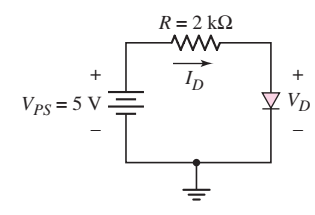
\includegraphics[width=\textwidth, height=9\baselineskip, keepaspectratio=true]{ds1}
\end{center}
\begin{equation}\scalebox{1.25}{
$
I_D = I_S (e^{\frac{V_D}{V_T}} - 1) = \frac{B_PS}{R} - \frac{V_D}{R}
$
}
\end{equation}
\begin{equation}\scalebox{1.25}{
$
V_{PS} = I_SR(e^{\frac{V_D}{nV_T}} - 1)+V_D
$
}
\end{equation}
\begin{equation}\scalebox{1.25}{
$
0.1A = (190nA)(e^{\frac{0.21V}{n\times 0.026V}} - 1) \implies n = \frac{0.21V}{ln(\frac{0.1A}{190nA}+1)(0.026V)} = 0.61
$
}
\end{equation}
The diode voltage is $V_D = 0.21$ and the diode current is $I_D=01.A$.
	
\subsection{Validation}

\begin{center}
LTSpice Implementation (accurate with $< 5\%$ deviation from design result)
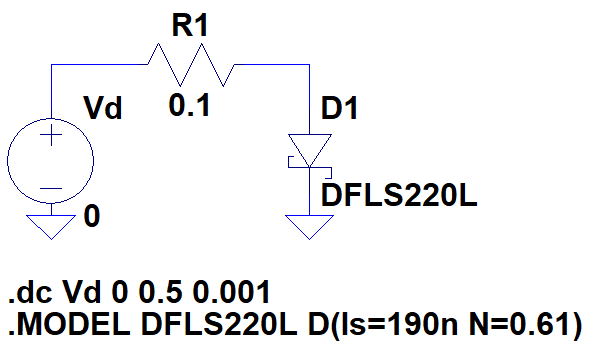
\includegraphics[width=.49\textwidth, height=\textheight, keepaspectratio=true]{ds1b}
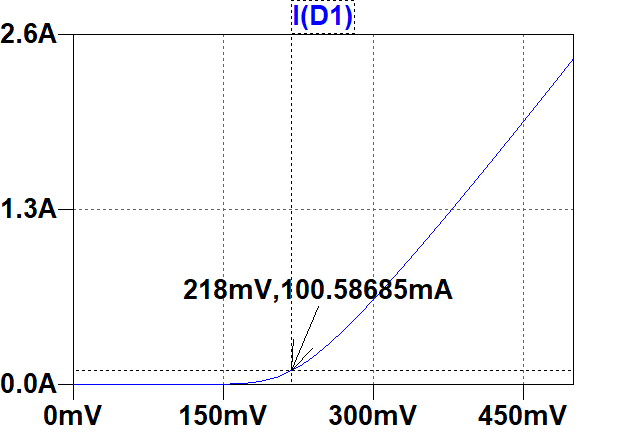
\includegraphics[width=.49\textwidth, height=\textheight, keepaspectratio=true]{ds1c}
$Err = \frac{|210-218|}{210} = 0.038 = 3.8\%$ The deviation is due to inaccuracies reading the charts on the datasheet.
\end{center}

\clearpage
\section{Problem 4.6.b.1: } Derived from 1.39 by changing values.
\subsection{Design}

Consider the following diode circuit with the following alternative values. $D=DFLS220L$, $R = 15k\Omega$, $\pm V = 3V$, $V_T = 0.026V$
\begin{center}
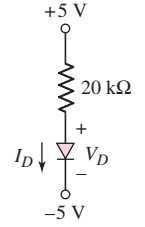
\includegraphics[width=\textwidth, height=7\baselineskip, keepaspectratio=true]{ds2}
\end{center}

The diode reverse saturation current is $I_S = 200nA$. Determine the diode current $I_D$ and diode voltage $V_D$. $I_D = 10mA$, $V_D = 0.15V$
\begin{equation}\scalebox{1.25}{
$
10mA = (200 nA)(e^{\frac{V_D}{n\times 0.026V}} - 1) \implies \frac{0.15V}{\ln(\frac{10mA}{200nA}+1)(0.026V)} = 0.53
$
}
\end{equation}

\subsection{Validation}

\begin{center}
LTSpice Implementation (accurate with $< 1\%$ deviation from design result)
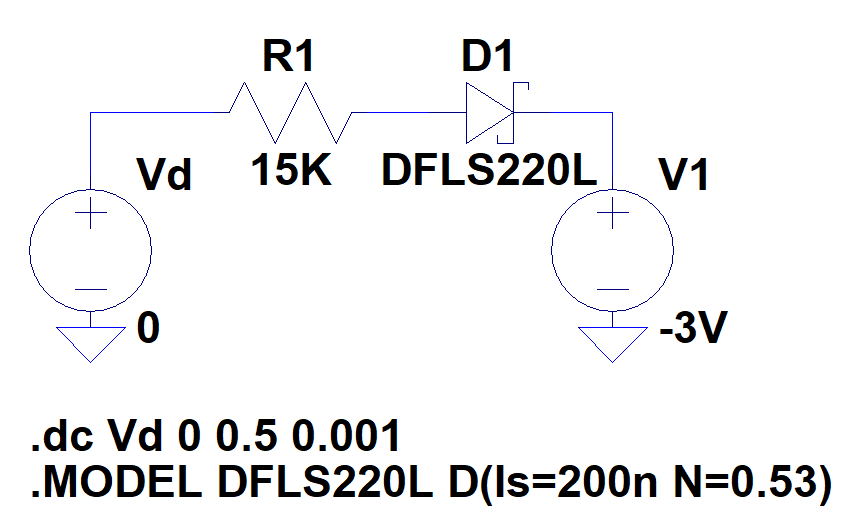
\includegraphics[width=.49\textwidth, height=\textheight, keepaspectratio=true]{ds2b}
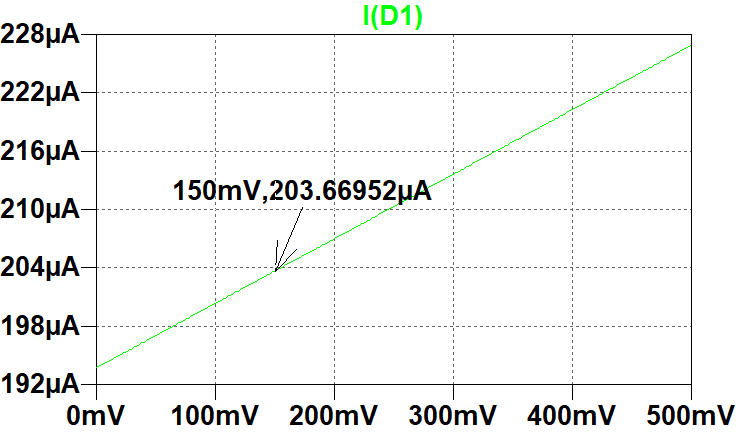
\includegraphics[width=.49\textwidth, height=\textheight, keepaspectratio=true]{ds2c}
$Err = \frac{|200-203.6|}{200} = 0.018 = 1.8\%$ The deviation is due to inaccuracies reading the charts on the datasheet.
\end{center}

This assignment demonstrates capability to analyse data sheets and perform basic analysis of diode circuits.

\textit{I have neither given nor received unauthorized assistance on this assignment.}


\end{raggedright}
\end{document}
